\section{Modelamiento Base de datos MongoDb}

\subsection{Modelo entidad relación}
Modelo entidad relación con retroalimentación dada en la entrega número 2.

\begin{figure}[H]
  \centering
  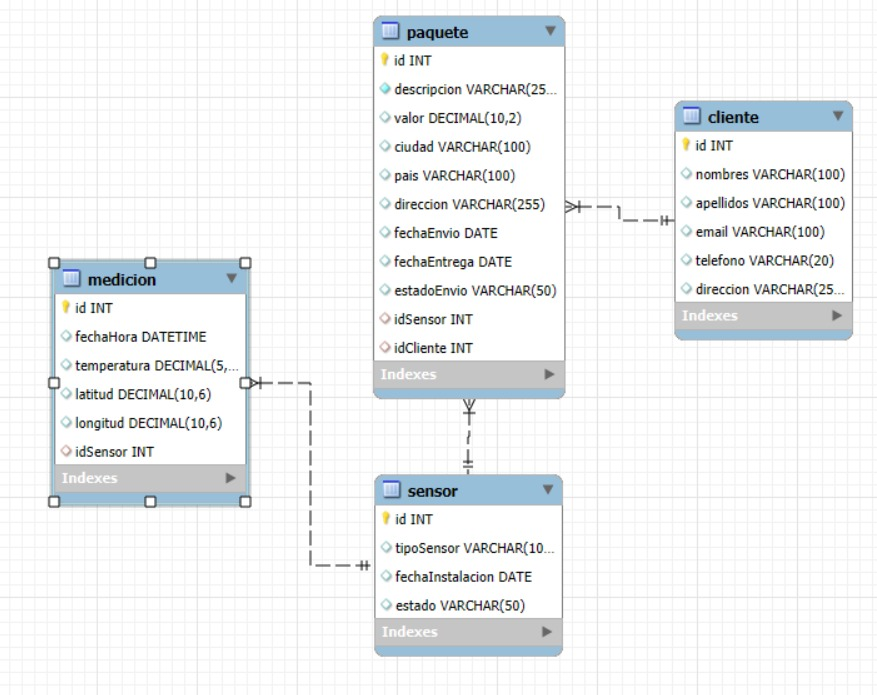
\includegraphics[width=0.9\textwidth]{Figures/1. Content/Modelo_ER.jpeg}
  \caption{Modelos Entidad Relación.}
  \label{fig:Modelo_ER}
\end{figure}

\subsection{Carga de trabajo}

\begin{table}[h!]
  \centering
  \renewcommand{\arraystretch}{2.5} % Ajusta la altura de las filas
  \begin{adjustbox}{width=\textwidth}
  \begin{tabular}{|p{2cm}|p{5cm}|p{3cm}|p{3cm}|p{3cm}|p{4cm}|}
  \hline
  \textbf{Tipo} & \textbf{Información} & \textbf{Frecuencia} & \textbf{Criticidad} & \textbf{Latencia} & \textbf{Tamaño} \\
  \hline
  Lectura & Cada entidad tiene un conjunto de operaciones CRUD. Las más importantes son las consultas en tiempo real de los estados de los sensores. & La lectura para clientes conectados es alta para la vista de métricas en tiempo real. & La lectura es crítica para las métricas, ya que su consulta es esencial para la empresa. & Mínima de 30 segundos, suficiente para el análisis de eventos relevantes. & Alcanzan su máximo cuando un cliente consulta información que supera el límite del BSON (Max: 16MB). \\
  \hline
  Escritura & Las creaciones de documentos son orgánicas, excepto para las mediciones. & Frecuencia alta debido a las mediciones automáticas constantes. & Es crítica porque una mala métrica puede implicar la pérdida de un paquete. & Mínima de 1 segundo por medición para mantener la calidad. & La escritura más relevante es la del paquete, pero en frecuencia, destacan las mediciones. \\
  \hline
  Lectura por pipeline & Involucra varias entidades en una consulta. & Frecuencia de una vez por conexión. & Facilita la navegación del cliente. & Máximo de 4 segundos para mantener una buena experiencia de usuario. & No supera el máximo de BSON debido al paginado implementado. \\
  \hline
  \end{tabular}
  \end{adjustbox}
  \caption{Carga de trabajo en el modelo MongoDB}
\end{table}

\subsection{Justificación del uso de documentos embebidos o referenciados}

\begin{figure}[H]
  \centering
  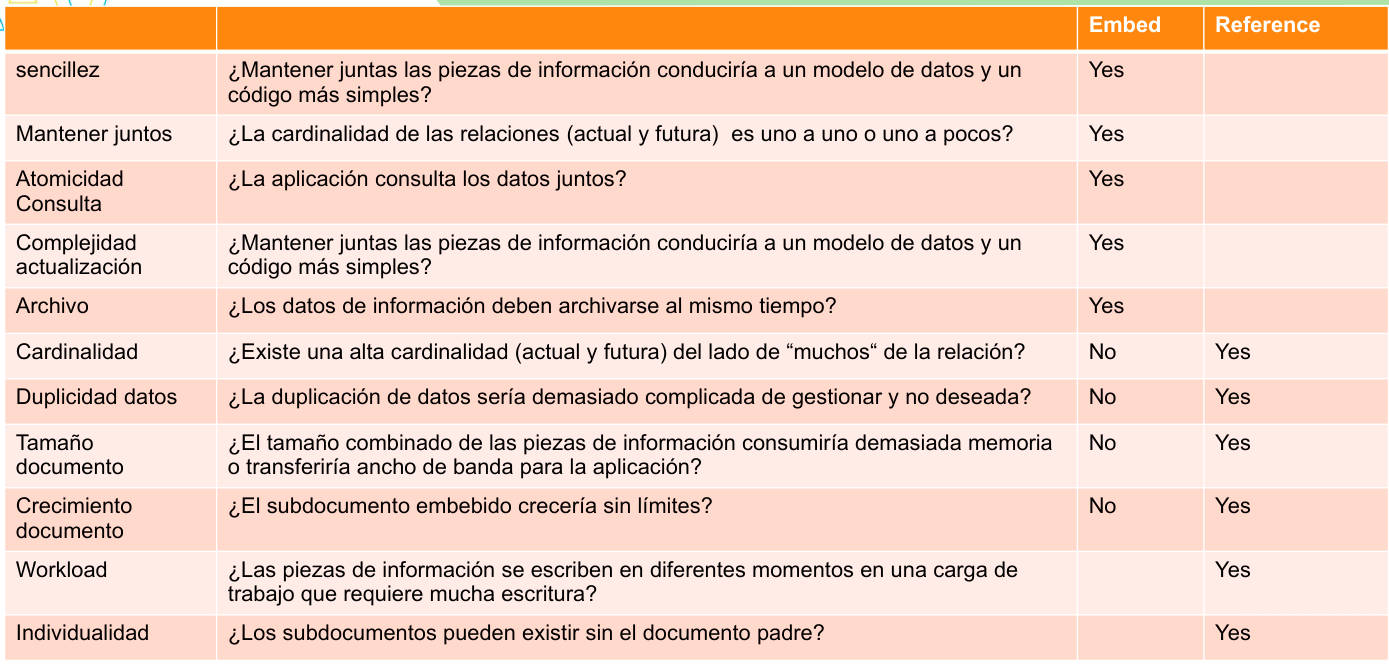
\includegraphics[width=\textwidth]{Figures/1. Content/Referenciado.png}
  \caption{Tabla comparativa}
  \label{fig:tabla_comparativa}
\end{figure}

Creando nuestro modelo a partir de esta tabla, encontramos que las mediciones deberían referenciar al sensor que las toma, y que los paquetes referencien al cliente propietario. La cantidad de variables ambientales medidas en un paquete no es tan alta, por lo que también se podría considerar embeber la entidad paquete con la entidad sensor para simplificar la distribución de información, aunque esto puede resultar en información innecesaria en algunas consultas.

\subsection{Patrón usado}
Inicialmente, optamos por el patrón Outlier. Sin embargo, tras una investigación profunda, decidimos cambiar al patrón de Árbol, que se adapta mejor al proyecto debido a su estructura jerárquica, permitiendo una organización y acceso eficiente de los datos.

\subsection{Creación Base de datos MongoDb}
Este \href{https://eafit-my.sharepoint.com/:f:/g/personal/jayoungh_eafit_edu_co/EuNCT-OUGs5DostAzMy--_YBnfqTibTuUjBO4LGQer7-HA?e=c67An0}{enlace del proyecto final} lleva a los JSON necesarios o los puedes ver en la entrega interactiva.

\begin{itemize}
  \item \href{https://eafit-my.sharepoint.com/:f:/g/personal/jayoungh_eafit_edu_co/EuNCT-OUGs5DostAzMy--_YBnfqTibTuUjBO4LGQer7-HA?e=c67An0}{Enlace.}
\end{itemize}


\subsection{Consulta MongoDb}
Ambas consultas incluyen \textbf{aggregate} y \textbf{lookup}:

\begin{itemize}
    \item Consulta 1: Busca todos los paquetes asociados a un tipo específico de sensor. 
    \begin{figure}[H]
      \centering
      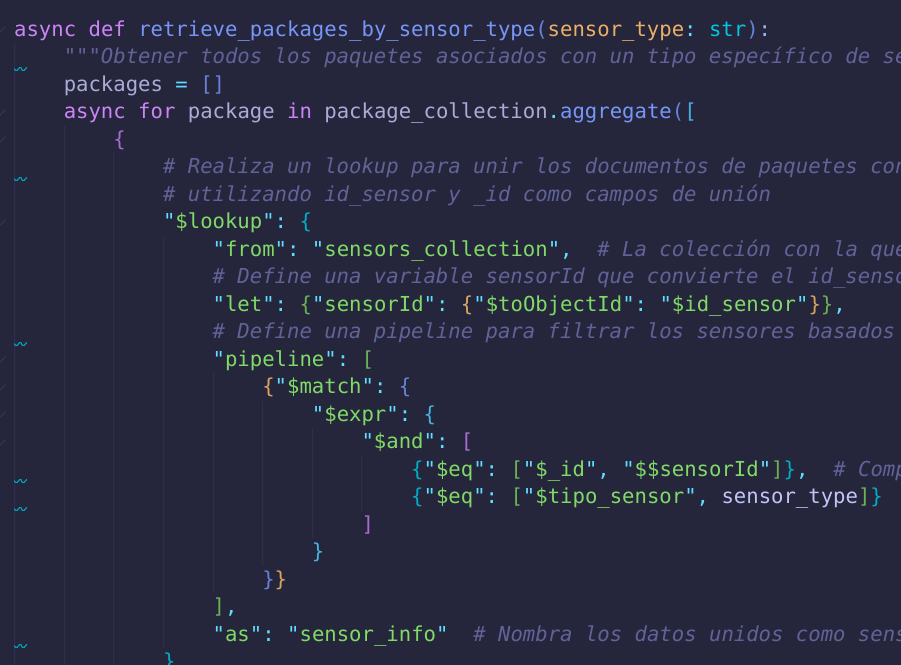
\includegraphics[width=0.9\textwidth]{Figures/1. Content/retrieve_packages_by_sensor_type.png}
      \caption{Paquetes asociados a un tipo específico de sensor.}
      \label{fig:retrieve_packages_by_sensor_type}
    \end{figure}

    \item Consulta 2: Busca todos los paquetes asociados a un usuario por su email.
      
  \begin{figure}[H]
    \centering
    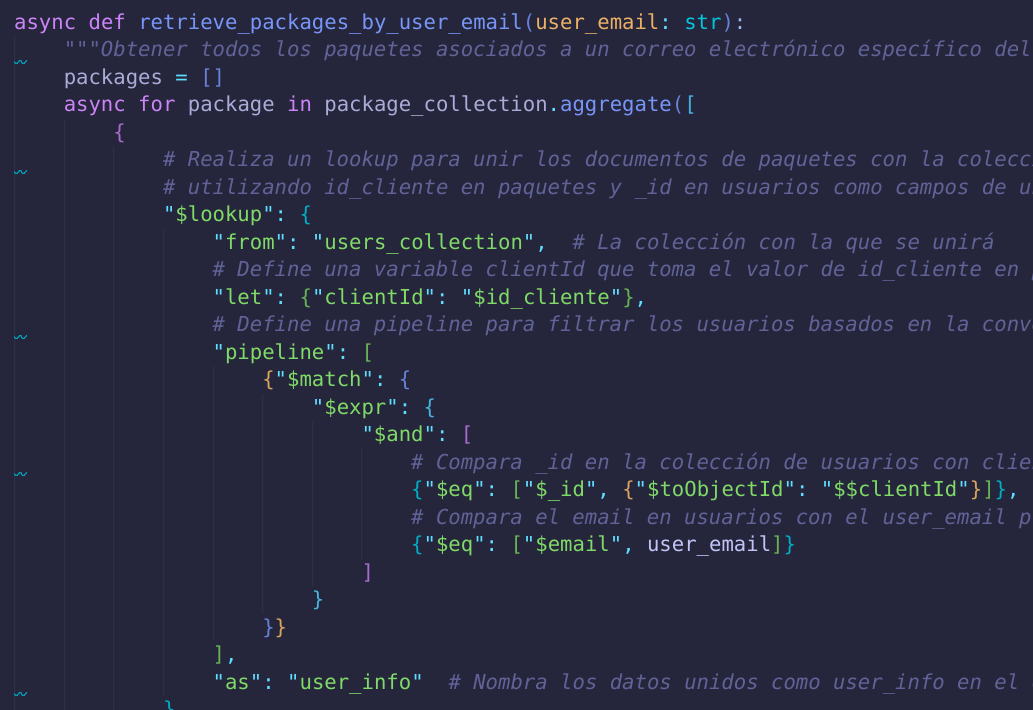
\includegraphics[width=0.9\textwidth]{Figures/1. Content/retrieve_packages_by_user_email.png}
    \caption{Paquetes asociados a un usuario por su email.}
    \label{fig:retrieve_packages_by_user_email}
  \end{figure}
\end{itemize}

\section{Conclusiones}

\begin{enumerate}
    \item \textbf{¿Qué es lo más relevante que se debe tener en cuenta en la elección de la base de datos de un proyecto?} \\
    Depende de la necesidad lo que se considere lo más relevante, pero sí hay una lista clave de cosas que forman parte de la elección de la base de datos para un proyecto y estas son:
    \begin{itemize}
        \item Modelo de los datos: estructurales y no estructurales.
        \item Escalabilidad: horizontal o vertical, es decir, si se amplía la infraestructura o se mejora la ya existente, respectivamente.
        \item Consistencia o disponibilidad.
        \item Soporte de integración.
        \item Costo.
    \end{itemize}
    
    \item \textbf{¿Qué aspecto es el que da más dificultad durante el proceso de diseño y la implementación de la base de datos?} \\
    El aspecto que suele generar más dificultad durante el diseño e implementación de una base de datos es encontrar el modelo de datos óptimo que garantice tanto el rendimiento como la escalabilidad, especialmente para aplicaciones con necesidades complejas de almacenamiento y acceso a datos, como en el caso de IoT.
    
    \item \textbf{¿Por qué son importantes las bases de datos o por qué no lo son?} \\
    Las bases de datos son muy importantes en la actualidad porque, en primer lugar, hacen posible el manejo de grandes volúmenes de datos, y no serían útiles para aplicaciones simples o temporales, datos de un solo uso o cuando hay alternativas aún más simples como archivos de texto.
    
    \item \textbf{¿Qué aspecto o tema generó más dificultad a la hora de realizar el proyecto?} \\
    Crear las relaciones, debido a que había que pensar en la lógica de negocio y en la escalabilidad simultáneamente debido a la poca planificación que involucra las bases de datos no relacionales.
    
    \item \textbf{¿Qué aprendizaje generó la realización del proyecto?} \\
    Nos dio un vistazo de muchos aspectos que no se tienen en cuenta cuando solo se indaga en las implementaciones de las tecnologías y nos dio una primera probada de lo sofisticado y hermoso que puede llegar a ser la creación de una buena base de datos y lo provechoso que es.
    
    \item \textbf{¿Qué lecciones aprendidas dejó la realización del proyecto? ¿Qué no deben hacer, qué se debe hacer, qué se debe mejorar en todo el proceso de diseño e implementación de base de datos?} \\
    Aprendimos que para lograr un buen diseño primero debemos planificar, y al momento de planificar hay que pensar en la implementación sin dejar de lado la lógica de negocio. También hay que entender bien cómo se forman las relaciones entre entidades, estando en todo momento con la certeza de la utilidad de las mismas. Jamás hay que comenzar codificando porque no se llegará a nada, y tampoco hay que pasar por alto la posibilidad de un crecimiento de la base de datos a futuro, ya que esto podría generar una deuda técnica.
    
    \item \textbf{Expectativas, temas y metodología de clase} \\
    Todas las expectativas del curso se cumplieron, y los temas que vimos fueron relevantes y bien seleccionados. No hubo temas que se sintieran innecesarios, y el contenido estuvo bien balanceado; agregar más podría restarles profundidad a los temas actuales. La metodología de la clase fue buena y ayudó a entender bien los contenidos.
\end{enumerate}

